\documentclass[a4paper,11pt,twoside]{article}
\usepackage{latexsym}
\usepackage[utf8]{inputenc}
\usepackage{lineno}
\usepackage{natbib}
\usepackage{geometry}
\RequirePackage{graphicx}
\RequirePackage{booktabs}
\RequirePackage[absolute]{textpos}

\usepackage[colorlinks,linkcolor={blue},citecolor={blue},urlcolor={red}]{hyperref}
\hypersetup{urlcolor=blue, colorlinks=true} % Colors hyperlinks in blue

\linespread{1.2} % Interlineado
\geometry{left=23mm, right=23mm, top=23mm, bottom=23mm} % Control de margenes

\title{Rapid forecasting of parametres of far field tsunamis for Peruvian coasts in real-time}
\author{Cesar Jimenez\\
 Universidad Nacional Mayor de San Marcos, Lima Perú \\
\emph{cjimenezt@unmsm.edu.pe}\\}

\begin{document}
%\linenumbers % Coloca numeracion a las lineas
\maketitle
%\logo{Orcid}
\begin{textblock*}{297mm}(80.3mm,60.8mm)
	\href{https://orcid.org/0000-0002-3671-4748}{
	\includegraphics[scale=0.033]{orcid}}
\end{textblock*}

\begin{abstract} \noindent
In this research, we have implemented an automatic software based on a linear tsunami numerical model to evaluate the parametres of far field tsunamis in the Pacific Ocean, such as tsunami travel time and maximum tsunami height. The computation time on a personal computer Intel i7 with Linux operative system using Intel Fortran parallel programming is around 30 minutes; the same process running on a supercomputer lasts around 2 minutes. Therefore, the usefulness of this software is on tsunami early warning, due to the tsunami travel time of far field tsunamis is greater than 5 or 6 hours and it is possible to conduct the tsunami simulation of the entire process.  \\ 
\textbf{Keywords}: tsunami, numerical simulation, tsunami warning.
\end{abstract}

\section*{Introduction}
In general, the tsunamis are classified, according to the tsunami travel time ($t_a$), in near field tsunamis when $t_a <$ 2 hours and far field tsunamis when $t_a >$ 5 hours. For tsunami early warning purposes, it is not possible to conduct a tsunami simulation in the case of near field tsunami because the reaction time is small.

%Este reporte preliminar de tsunami de origen lejano ha sido elaborado en forma automática por el modelo numérico TSDHN-2022.

\subsection*{Background of previous research}
%\cite{Sil1978} reported t
In this research, .

\cite{Wan2012} developed an experimental real-time inundation forecasting of tsunamis (RIFT) model, to complement the pre-computed database approach.



\section*{Methodology}
Las dimensiones de la fuente sísmica se calculan a partir de las ecuaciones de \cite{Pap2004}. El mecanismo focal del terremoto se toma de la base de datos del Global CMT. El campo de deformación se obtiene a partir de las ecuaciones analíticas de \cite{Oka1992}.

La simulación de la propagación del tsunami se realiza con el modelo numérico TUNAMI, modelo lineal y en coordenadas esféricas \citep{Ima2006}. La grilla batimétrica computacional abarca todo el Océano Pacífico, con una resolución de 4 min o 240 s. El cálculo de las isócronas de tiempos de arribo para todo el Océano Pacífico se realizó con el modelo Tsunami Travel Time \citep{Wes2009}. 

Se han colocado 3 mareógrafos virtuales en los puertos de Talara, Callao y 
Matarani. Se utilizó la ley de Green para la corrección de la amplitud de 
los mareogramas, debido a que los nodos computacionales no coinciden 
necesariamente con la ubicación de las estaciones mareográficas costeras \citep{Sat2015}.

El tiempo promedio de cómputo para una PC i7 es de 15 min para una ventana 
de tiempo de simulación de 28 horas (Figura 1). Sin embargo, el 
supercomputador DHN demora menos de 2 minutos. \\

\noindent \textbf{Nota:} El resultado del modelo TSDHN-2022 es una estimacion referencial y de preferencia debe ser utilizado para obtener los parámetros de tsunamis de origen lejano, es decir fuera de las fronteras del litoral de Perú. Para eventos de origen cercano, se debe utilizar el modelo Pre-Tsunami \citep{Jim2018}.

\section*{Results and Discussion}
La Tabla 1 muestra los parámetros hipocentrales y el mecanismo focal del terremoto. La Figura 1 muestra el mapa de propagacion de la máxima energía, la ubicación del epicentro está representado por la esfera focal y las estaciones mareográficas están representadas por los triángulos azules

La Figura 2 muestra los mareogramas simulados para las estaciones del litoral del Perú, de norte a sur: Talara, Callao y Matarani. La Tabla 2 muestra los tiempos de arribo y la máxima altura del tsunami en las estaciones mareográficas del litoral peruano.

\begin{table*}
	\centerline{
		\begin{tabular}[t]{lp{0.5cm}l}
			\toprule
			Parámetro   & & Valor \\
			\midrule
			Latitud     & &    0.95$^\circ$  \\
			Longitud    & &  -79.37$^\circ$  \\
			Profundidad & &   20.0 km       \\
			Magnitud    & &    8.8 Mw       \\
			\midrule
			Strike      & &   27.0$^\circ$  \\
			Dip         & &   15.0$^\circ$  \\
			Rake        & &   90.0$^\circ$  \\
			\bottomrule
	\end{tabular}}
	\caption{Parámetros hipocentrales y mecanismo focal del terremoto.}
\end{table*}

\begin{figure}
	\centerline{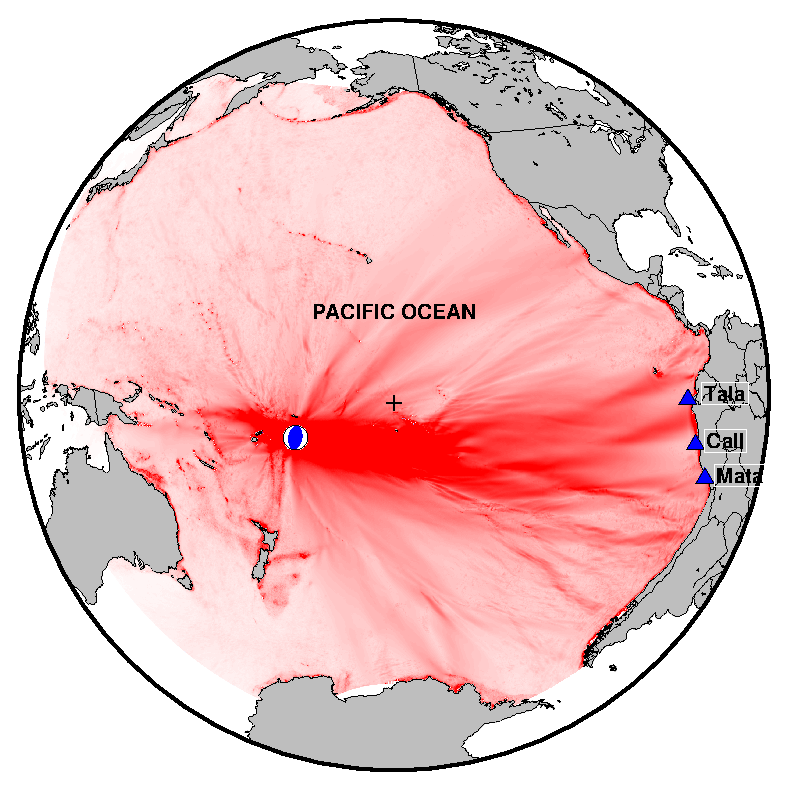
\includegraphics[scale=0.82]{maxola.eps}}
	\caption{Mapa de máxima altura de propagación del tsunami. La esfera focal representa el epicentro. Los triángulos azules representan a las estaciones mareográficas.}
	\label{mareograma}
\end{figure}

\begin{figure}
	\centerline{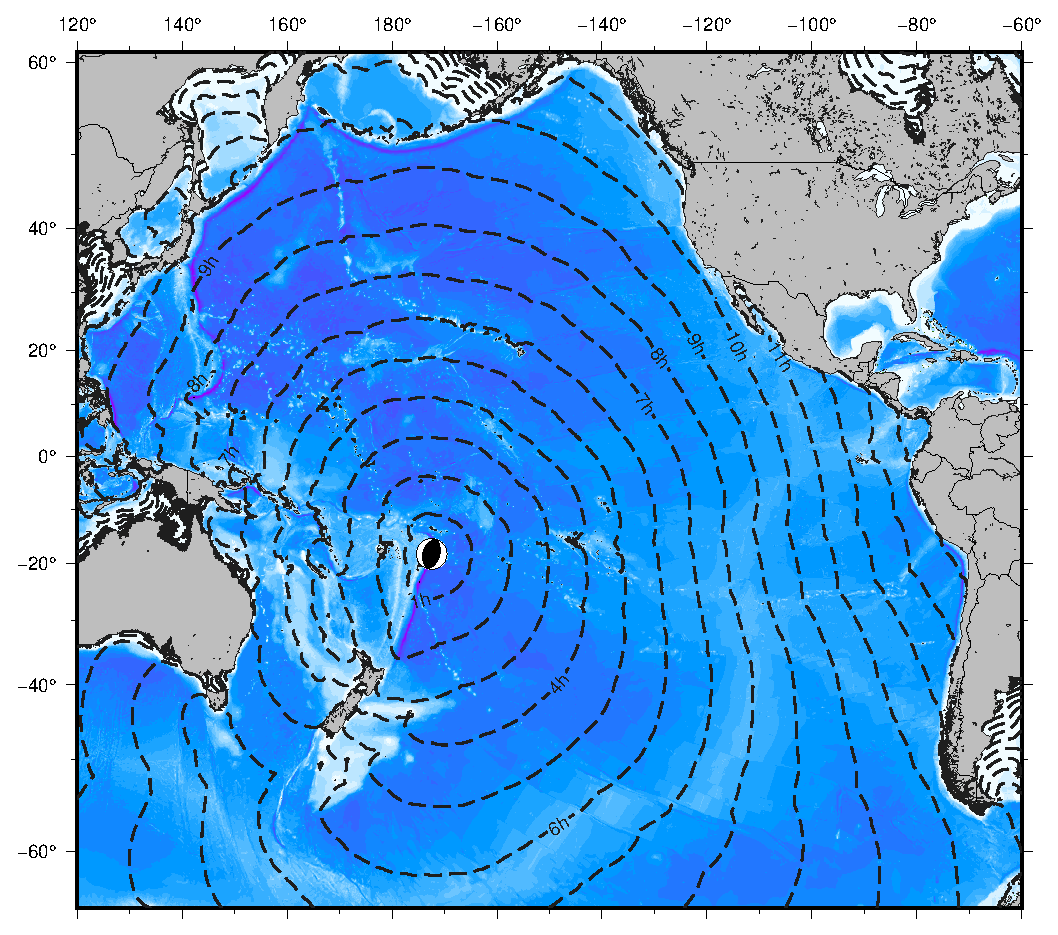
\includegraphics[scale=0.78]{ttt.eps}}
	\caption{Mapa de tiempo de arribo del tsunami. La esfera focal representa el 
		epicentro.}
	\label{ttt}
\end{figure}

\begin{figure}
	\centerline{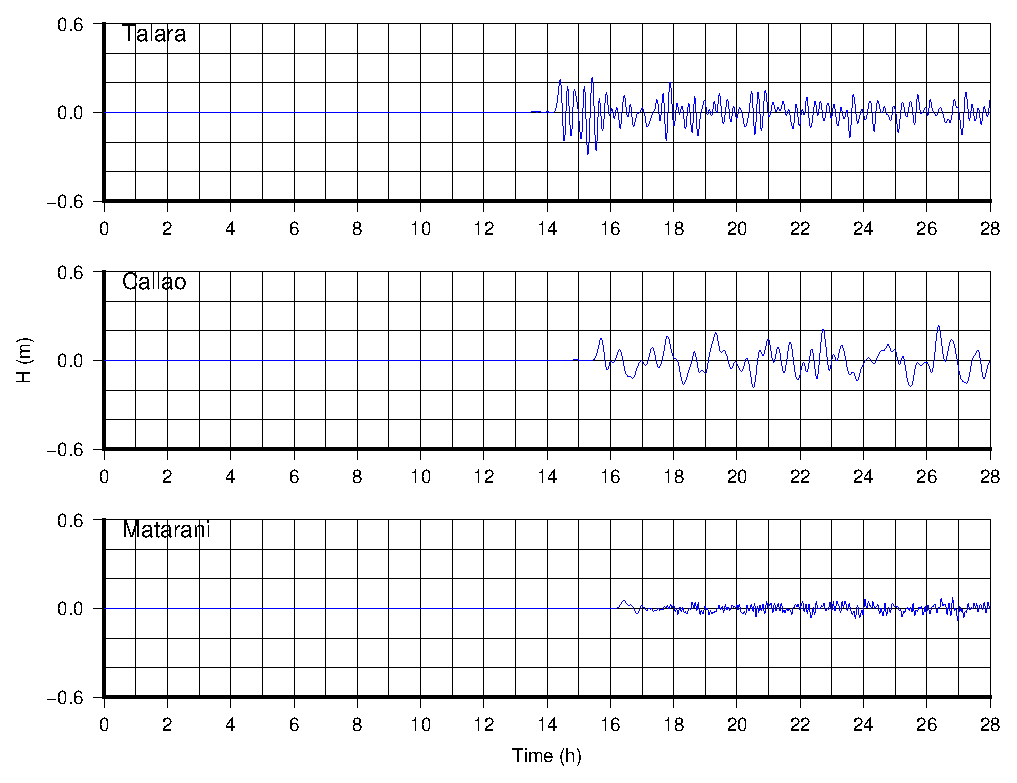
\includegraphics[scale=0.82]{mareograma.eps}}
	\caption{Simulated tsunami waveforms at the tidal stations of Talara, Callao and Matarani.}
\end{figure}

\begin{table*}
	\centerline{
		\begin{tabular}[t]{lcc}
			\toprule
			Estación     & Tiempo de arribo & Máximo (m) \\
			\midrule
			Talara     & 0:27 &   0.62  \\
			Callao     & 2:45 &   0.47  \\
			Matarani   & 3:36 &   0.21  \\
			\bottomrule
	\end{tabular}}
	\caption{Tiempo de arribo (hh:mm) y máxima amplitud del tsunami.}
\end{table*}

\section*{Conclusions}


\section*{Acknowledgements}
We are greatful with Mr. Xxxxx Xxxxx by the revision of the lingüistic aspects of the manuscript. Furthermore, we thank the research grant from the Universidad Nacional Mayor de San Marcos and from Concytec (Consejo Nacional de Ciencia, Tecnología e Innovación Tecnológica) of Peru.

\bibliographystyle{apalike}
\bibliography{referencias}

\end{document}
